\documentclass[12pt,a4paper]{article}
\usepackage{graphicx}
\usepackage{booktabs}
\usepackage{hyperref}


\begin{document}
\begin{titlepage}
	\centering
	
\includegraphics[width=0.4\textwidth]{courseraLogo}\par\vspace{3cm}
	{\scshape\large Applied Data Science Capstone Project \par}
	\vspace{1cm}
	{\scshape\LARGE The Battle of Neighborhoods\par}
%	\vfill
%	supervised by\par
%	Dr.~Mark \textsc{Brown}
	\vfill
	{\large \today\par}
\end{titlepage}
\section{Introduction}
A chain of vegetarian/vegan restaurants based in North America is looking into expanding to Europe. They have asked for a report on vegetarianism/veganism in the capitals of Europe to decide which European cities to start with. 

This report will present a number of relevant statistics for European countries and their capitals. This includes the number of vegetarians/vegans as part of their population, the number of current vegetarian/vegan restaurants in their city centers, and the disposable income of households in each country. Based on this data, cities where the client's chain of vegetarian/vegan restaurants are likely to succeed will be identified.

This report will start with a description of the data used for this investigation in Section~\ref{sec:data}. Next, the methodology for the exploratory data analysis, statistical testing and machine learning techniques are explained in Section~\ref{sec:methodology}. Results are presented in Section~\ref{sec:results}, after which the report concludes with the discussion and conclusion in Sections~\ref{sec:discussion} and \ref{sec:conclusion}, respectively.

\section{Data}
\label{sec:data}
Countries that are investigated are given in Table~\ref{tab:countriescapitals}. To be able to use Foursquare to obtain information on venues in these capitals, the latitude and longitude for these cities is also required. The center of each city is obtained from a dataset containing the latitude and longitude of many cities from \url{simplemaps.com} \cite{latlong}. The city center is defined as a circle with a diameter of 3 km around the center of the city. The latitude and longitude, as obtained from Ref.~\cite{latlong}, can also be found in the last two columns of Table~\ref{tab:countriescapitals}. The cities are shown in Fig.~\ref{fig:cities}. 

Data used for clustering of the cities in this study are the following:
\begin{enumerate}
	\item Proportion of vegetarian/vegan individuals in the population. To be obtained from the Wikipedia-page "Vegetarianism by country" \cite{wikiVega}. Data is available for all countries, except for the number of vegans in Austria. This value will therefore be approximated using the available data. 
	\item Current number of vegetarian/vegan restaurants in a circle of 3 km diameter around the center of the city. To be obtained using Foursquare data. Because Foursquare calls are limited to 100 results, the diameter of the circle cannot be increased for this study. On a similar note, ideally this study would look at the \textit{proportion} of these restaurants out of all restaurants, but this will go well over the limit for Foursquare unfortunately. 
	\item Median disposable income per household. To be obtained from the Wikipedia-page "Disposable household and per capita income" \cite{wikiIncome}. Data is available for all countries. 
\end{enumerate}
Wherever data is obtained for a country rather than just the city, it is assumed that this value is a sufficient approximation for the data of the city. 

The obtained data is compiled in Table~\ref{tab:data}. Inspecting the data shows no extreme outliers and the only missing value, proportion of vegans in Austria, has been calculated using a Linear Regression model. While the number of reported vegetarian/vegan restaurants in Bern and Lisbon appears low, this can be explained by the relatively low number of vegetarians/vegans in those countries, so this does not necessarily mean that these numbers are inaccurate. The reader is referred to the Jupyter Notebook attached to this report to see how the data has been obtained through webscraping and Foursquare. 

\begin{table}[htbp!]
	\centering
	\caption{Countries the client is interested in, along with their capital city and latitude and longitude \cite{latlong}.}
	\label{tab:countriescapitals}
	\begin{tabular}{llll}
		\toprule
		\textbf{Country} 	& \textbf{Capital}  & \textbf{Latitude, $^{\circ}$} & \textbf{Longitude, $^{\circ}$} \\ \midrule
		Austria				& Vienna			& 48.2083			&	16.3731		\\
		Belgium 			& Brussels			& 50.8467			&	4.3517\\
		Czech Republic 		& Prague  			& 50.0833			&	14.4167\\
		Denmark 			& Copenhagen 		& 55.6786			&	12.5635\\
		Finland 			& Helsinki  		& 60.1756			&	24.9342\\
		France 				& Paris 			& 48.8566			&	2.3522\\
		Germany 			& Berlin 			& 52.5167			&	13.3833\\
		Italy 				& Rome 				& 41.8931			&	12.4828\\
		Ireland 			& Dublin    		& 53.3425			&	-6.2658\\
		Netherlands	 		& Amsterdam 		& 52.3500			&	4.9166\\
		Norway 				& Oslo 				& 59.9111			&	10.7528\\
		Poland 				& Warsaw   			& 52.2167			&	21.0333\\
		Portugal 			& Lisbon 			& 38.7452			&	-9.1604\\
		Spain 				& Madrid 			& 40.4189			&	-3.6919\\
		Sweden 				& Stockholm 		& 59.3294			&	18.0686\\
		Switzerland 		& Bern 				& 46.9480			&	7.4474\\
		United Kingdom 		& London 			& 51.5072			&	-0.1275\\ 
		\bottomrule
	\end{tabular}
\end{table}
\begin{figure}
	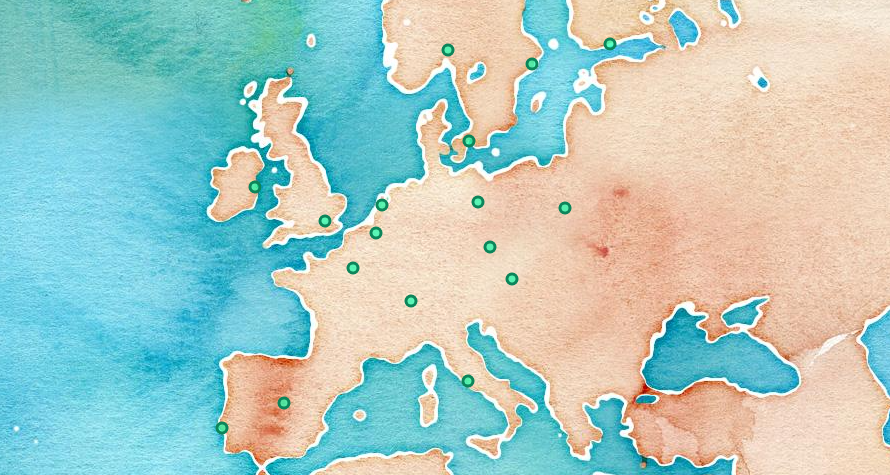
\includegraphics[width=\linewidth]{cities}
	\caption{Capital cities of Europe of interest to the client. }
	\label{fig:cities}
\end{figure}

\begin{table}[htbp!]
	\centering
	\caption{Obtained data for each country/capital.}
	\label{tab:data}
	\scalebox{0.85}{\begin{tabular}{llp{2.5cm}p{2.5cm}p{2.5cm}p{2.1cm}}
		\toprule
		\textbf{Country} 	& \textbf{Capital}  & \textbf{Percentage of vegetarians, \%} & \textbf{Percentage of vegans, \%} & \textbf{Number of vegetarian restaurants, -} & \textbf{Disposable income, \$} \\ \midrule
		Austria			& Vienna	& 10.0	& 2.8 & 	61 & 	32496 \\ 
		Belgium			& Brussels	& 7.0	& 1.0 & 	55 & 	29361 \\ 
		Czech Republic	& Prague	& 5.0	& 1.0 & 	70 & 	17984 \\ 
		Denmark			& Copenhagen& 10.0	& 4.0 & 	71 & 	28926 \\ 
		Finland			& Helsinki	& 11.0	& 2.0 & 	95 & 	26774 \\ 
		France			& Paris		& 5.2	& 1.1 & 	67 & 	25865 \\ 
		Germany			& Berlin	& 12.0	& 2.0 & 	57 & 	27569 \\ 
		Italy			& Rome		& 8.9	& 2.2 & 	36 & 	23023 \\ 
		Ireland			& Dublin	& 8.4	& 2.0 & 	47 & 	25933 \\ 
		Netherlands		& Amsterdam	& 5.0	& 1.0 & 	23 & 	29571 \\ 
		Norway			& Oslo		& 9.0	& 4.0 & 	19 & 	35542 \\ 
		Poland			& Warsaw	& 8.4	& 7.0 & 	23 & 	16507 \\ 
		Portugal		& Lisbon	& 1.2	& 0.6 & 	11 & 	15403 \\ 
		Spain			& Madrid	& 1.5	& 0.2 & 	62 & 	21788 \\ 
		Sweden			& Stockholm	& 12.0	& 4.0 & 	65 & 	29765 \\ 
		Switzerland		& Bern		& 5.0	& 1.0 & 	9  & 	37749 \\ 
		United Kingdom	& London	& 21.3	& 4.4 &    100 & 	22603 \\ 
		\bottomrule
	\end{tabular}}
\end{table}

\section{Methodology}
\label{sec:methodology}
Machine learning techniques used in this study are \textbf{Linear Regression}, \textbf{Robust Scaling} and \textbf{K-Means Clustering}. This section will briefly introduce these methods. 

As mentioned in Section~\ref{sec:data}, the missing data in the feature set has been calculated using a Linear Regression model. Training data for the model is from all cities other than Vienna, with \texttt{X} as the number of vegetarians in each city and \texttt{y} as the number of vegans in each city. No other features are used in this model as they are not thought to be related to the target value (i.e. the latitude/longitude). 

The cities are clustered using a K-Means algorithm, which clusters the data based on a set of features. These features are first scaled, since otherwise the clustering would almost exclusively be based on the "disposable income"-feature, which is orders of magnitude larger than the other features. Robust Scaling from the scikit-learn preprocessing toolbox is used to perform this scaling. The K-Means algorithm separates the samples in $k$ groups, minimizing the within-cluster sum-of-squares of the features. Because of the limited number of cities included in this study, they will be clustered in $ k = 5$ groups. 

\section{Results}
\label{sec:results}
The clusters obtained by the K-Means algorithm are visualized in Fig.~\ref{fig:clusteredCities}. The data for the clustered cities is presented in Tables~\ref{tab:cluster0}-\ref{tab:cluster4}, for cluster 0 to 4, respectively (numbered in true Python fashion). 
\begin{figure}
	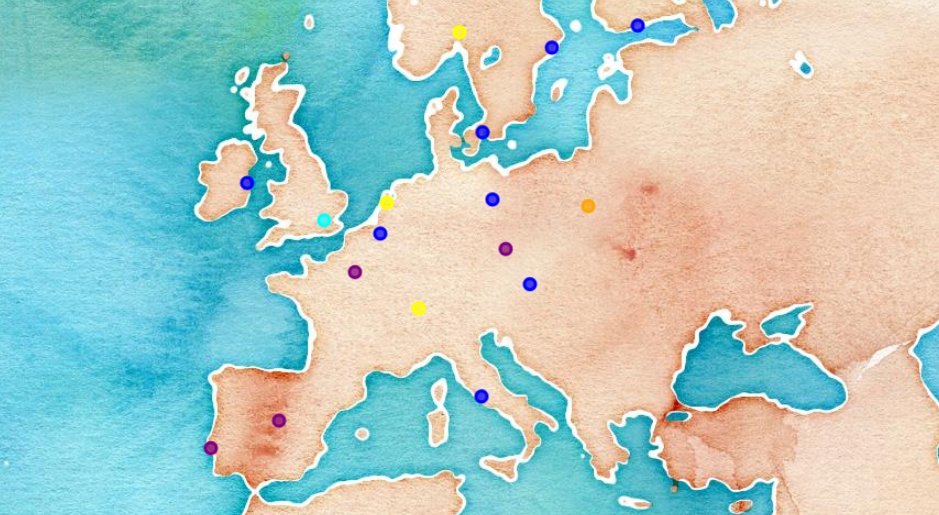
\includegraphics[width=\linewidth]{clusteredCities}
	\caption{Clustered cities in Europe. }
	\label{fig:clusteredCities}
\end{figure}

\begin{table}[htbp!]
	\centering
	\caption{Cities in cluster 0.}
	\label{tab:cluster0}
	\scalebox{0.85}{\begin{tabular}{llp{2.5cm}p{2.5cm}p{2.5cm}p{2.1cm}}
			\toprule
			\textbf{Country} 	& \textbf{Capital}  & \textbf{Percentage of vegetarians, \%} & \textbf{Percentage of vegans, \%} & \textbf{Number of vegetarian restaurants, -} & \textbf{Disposable income, \$} \\ \midrule
			Czech Republic	& Prague	& 5.0	& 1.0 & 	70 & 	17984 \\ 
			France			& Paris		& 5.2	& 1.1 & 	67 & 	25865 \\ 
			Portugal		& Lisbon	& 1.2	& 0.6 & 	11 & 	15403 \\ 
			Spain			& Madrid	& 1.5	& 0.2 & 	62 & 	21788 \\ 
			\bottomrule
	\end{tabular}}
\end{table}

\begin{table}[htbp!]
	\centering
	\caption{Cities in cluster 1}
	\label{tab:cluster1}
	\scalebox{0.85}{\begin{tabular}{llp{2.5cm}p{2.5cm}p{2.5cm}p{2.1cm}}
			\toprule
			\textbf{Country} 	& \textbf{Capital}  & \textbf{Percentage of vegetarians, \%} & \textbf{Percentage of vegans, \%} & \textbf{Number of vegetarian restaurants, -} & \textbf{Disposable income, \$} \\ \midrule
			Austria			& Vienna	& 10.0	& 2.8 & 	61 & 	32496 \\ 
			Belgium			& Brussels	& 7.0	& 1.0 & 	55 & 	29361 \\ 
			Denmark			& Copenhagen& 10.0	& 4.0 & 	71 & 	28926 \\ 
			Finland			& Helsinki	& 11.0	& 2.0 & 	95 & 	26774 \\ 
			Germany			& Berlin	& 12.0	& 2.0 & 	57 & 	27569 \\ 
			Italy			& Rome		& 8.9	& 2.2 & 	36 & 	23023 \\ 
			Ireland			& Dublin	& 8.4	& 2.0 & 	47 & 	25933 \\ 
			Sweden			& Stockholm	& 12.0	& 4.0 & 	65 & 	29765 \\ 
			\bottomrule
	\end{tabular}}
\end{table}

\begin{table}[htbp!]
	\centering
	\caption{Cities in cluster 2}
	\label{tab:cluster2}
	\scalebox{0.85}{\begin{tabular}{llp{2.5cm}p{2.5cm}p{2.5cm}p{2.1cm}}
			\toprule
			\textbf{Country} 	& \textbf{Capital}  & \textbf{Percentage of vegetarians, \%} & \textbf{Percentage of vegans, \%} & \textbf{Number of vegetarian restaurants, -} & \textbf{Disposable income, \$} \\ \midrule
			United Kingdom	& London	& 21.3	& 4.4 &    100 & 	22603 \\ 
			\bottomrule
	\end{tabular}}
\end{table}

\begin{table}[htbp!]
	\centering
	\caption{Cities in cluster 3}
	\label{tab:cluster3}
	\scalebox{0.85}{\begin{tabular}{llp{2.5cm}p{2.5cm}p{2.5cm}p{2.1cm}}
			\toprule
			\textbf{Country} 	& \textbf{Capital}  & \textbf{Percentage of vegetarians, \%} & \textbf{Percentage of vegans, \%} & \textbf{Number of vegetarian restaurants, -} & \textbf{Disposable income, \$} \\ \midrule
			Netherlands		& Amsterdam	& 5.0	& 1.0 & 	23 & 	29571 \\ 
			Norway			& Oslo		& 9.0	& 4.0 & 	19 & 	35542 \\ 
			Switzerland		& Bern		& 5.0	& 1.0 & 	9  & 	37749 \\ 
			\bottomrule
	\end{tabular}}
\end{table}

\begin{table}[htbp!]
	\centering
	\caption{Cities in cluster 4}
	\label{tab:cluster4}
	\scalebox{0.85}{\begin{tabular}{llp{2.5cm}p{2.5cm}p{2.5cm}p{2.1cm}}
			\toprule
			\textbf{Country} 	& \textbf{Capital}  & \textbf{Percentage of vegetarians, \%} & \textbf{Percentage of vegans, \%} & \textbf{Number of vegetarian restaurants, -} & \textbf{Disposable income, \$} \\ \midrule
			Poland			& Warsaw	& 8.4	& 7.0 & 	23 & 	16507 \\ 
			\bottomrule
	\end{tabular}}
\end{table}

\section{Discussion}
\label{sec:discussion}
Based on the data in Tables~\ref{tab:cluster0}-\ref{tab:cluster4}, the clusters can be described as:
\begin{enumerate}
	\item Cluster 0 contains the cities with low numbers of vegetarians and vegans, as well as relatively low disposable income, the number of vegetarian/vegan restaurants is medium for most cities in this cluster.
	\item Cluster 1 contains the cities with a high percentage of vegetarians and vegans, a medium-to-high number of current vegetarian restaurants and a medium-to-high disposable income.
	\item Cluster 2 contains the city with a very high number of vegetarians and vegans, a current number of vegetarian/vegan restaurants that is at the limit of what Foursquare can offer (so it is likely even higher!) and a medium disposable income.
	\item Cluster 3 contains the cities with a low-to-medium number of vegetarians and vegans, a low number of vegetarian restaurants and a high disposable income.
	\item The last cluster, Cluster 4, contains one city with a medium number of vegetarians, low number of current vegetarian/vegan restaurants and the lowest disposable income.
\end{enumerate}

Cities more suitable for the client's first European vegetarian/vegan restaurants can be found in clusters 1 and 2. Especially cluster 2, consisting of just London, is a great place to start with a new vegetarian/vegan restaurant, due to the very high number of vegetarians/vegans and the high number of current vegetarian/vegan restaurants indicates that the client's restaurant is likely to succeed here too.

Cluster 0 is less suitable because there is both a relatively low number of vegetarians and vegans and the disposable income is relatively low. Cluster 3 is less suitable because it has a relatively low-to-medium number of vegetarians and vegans and despite a high income, there are currently not many vegetarian/vegan restaurants, possibly indicating that these are not likely to succeed in these cities. Cluster 4 is less suitable because despite the medium number of vegetarians and vegans, the lowest disposable income of the cities in this study is a likely cause for the low number of current vegetarian/vegan restaurants, indicating that the client's restaurant is less likely to succeed here too. 


\section{Conclusion}
\label{sec:conclusion}
For an expansion from North America to Europe for our client, we advise that they start their first restaurant in London, United Kingdom. If this restaurant proves a success among Europeans, the advise is that the client expands further to Vienna, Brussels, Copenhagen, Helsinki, Berlin, Rome, Dublin and Stockholm. Especially with vegetarianism/veganism on the rise \cite{wikiVega} among younger people, we expect the client to successfully expand their business into Europe. 

\section{Future recommendations}
This study has been limited by the limits imposed by Foursquare. The imposed limit means that the circle of 3-km diameter cannot be increased to obtain the number of current vegetarian/vegan restaurants. Similarly, ideally this study would look at the \textit{proportion} of these restaurants out of all restaurants, but this number will go well over the limit for Foursquare. 

Other features that are ideally to be included in this study is the change in the proportion of vegetarians/vegans over time. Since this is on the rise, especially among young people \cite{wikiVega}, this information would be a great indicator to spot trendy cities for vegans. 


\newpage
\appendix
\bibliographystyle{ieeetr} 
\bibliography{bib}


\end{document}          
